% 
% ======================================================================
\RequirePackage{docswitch}
% \flag is set by the user, through the makefile:
%    make note
%    make apj
% etc.
\setjournal{\flag}

\documentclass[\docopts]{\docclass}

% You could also define the document class directly
%\documentclass[]{emulateapj}

% Custom commands from LSST DESC, see texmf/styles/lsstdesc_macros.sty
\usepackage{lsstdesc_macros}
\usepackage[utf8]{inputenc}
\usepackage{graphicx}
\usepackage{subfigure}
\graphicspath{{./}{./figures/}}
\bibliographystyle{apj}

% Add your own macros here:



% 
% ======================================================================

\begin{document}

\title{ Impact of the calibration on the performances of the LSST SN survey }

\maketitlepre

\begin{abstract}
The goal of the forecast work presented in this note is to study the impact of the LSST SN survey calibration, that is parametrized on one side as errors in the zeropoint of each filter ($\delta_{zp}$'s) and on the other as shifts in wavelength of each filter ($\delta_\lambda$'s) on the accuracy of the cosmology we will extract from LSST.
It is also a part of a proposed analysis pipeline in which the standardization of the SNe Ia, their spectrophotometric evolution and the cosmology are fitted at the same time.
\end{abstract}

% Keywords are ignored in the LSST DESC Note style:
\dockeys{photometry: calibration}

\maketitlepost

% ----------------------------------------------------------------------
% 

\section{Introduction}
\label{sec:intro}

% As we are getting closer to the first light of the Large Synoptic Survey Telescope, which will allow us to find and measure a huge amount of Type Ia Supernovae, the question of our preparation in order to extract the maximum of information on the dark energy from this future dataset is becoming crucial.
% One of the must critical point is about how we are able to reduce the systematics of the survey, and especially the calibration uncertainties.
%In section \ref{sec::jla} we present the state of the art in SNe Ia survey analysis through the Joint Light-curve Analysis (CITATION ARTICLE MARC), analysis of which the cosmology group of the LPNHE is familiar to.
%It will show that even for for a dataset that contains 100 times statistics the calibration has became one on the highest concerns.
In section \ref{sec::simulated_dataset} we rely on the work presented in (REF NOTE ON THE CADENCE OF ...) DESC note to highlight the observing cadence, the instrument and the observing conditions we use in this forecast work.
In \ref{ssec:snsim} we also rely on the work presented in (REF SNSIM ...) to explain how SNe Ia light curves are simulated here and the complete the full description of the dataset that will be the input of our analysis.
In \ref{sec::analysis_model} we focus on how the simulated dataset can be modelized using simultaneously the standardization of the SNe Ia, their photometric evolution through a SALT2-like model, and the cosmology.
In \ref{sec::calib_uncertainties} we explain how the calibration uncertainties are modelized and how they fit into the the model presented in \ref{sec::analysis_model}.
Emphasis will be put on how the two different sets of calibration parameters are connected and how it shapes the calibration covariance matrix, which will be expressed.
Finaly in section \ref{sec::results} we show how we quickly compute the performances of the survey through the calculus of the Figure of Merit (FoM), this for different calibration strategies.
In particular we show the example of the impact of the constrains on the calibration that the STARDICE experiment will put.
We also show the results given by this study trained on the JLA dataset to proove its reliability.
In \ref{sec::discussion} we discuss the results and compare them to those we obtain without taking into account the training of the SNe Ia spectrophotometric model.
We conclude in \ref{sec::conclusion}.

% ----------------------------------------------------------------------

% \section{State of the art : JLA}
% \label{sec::jla}

% Présentation des résultats JLA, description de la calibration \\
% Comparaison entre l'impact des systématiques et celui des incertitudes statistiques \\
% Ouverture sur la stat de LSST: super statistique gâchée si pas d'amélioration sur les systématiques, dont la principale est la calibration \\
% Demande une assez grosse discussion avec le groupe pour savoir ce que l'on met dans cette partie

% ----------------------------------------------------------------------

\section{Simulated dataset}
\label{sec::simulated_dataset}

\subsection{Cadence}
\label{subsec::cadence}

The LSST SN survey will be splitted in two different layers:
\begin{itemize}
\item A wide survey that will be composed of small time exposures over a large fraction of the sky.
  It would allow to discover a large number of nearby SNe Ia.
\item A deep survey inwhich a small number of fields will be observed but with high exposure times to ensure we get distant SNe Ia.
\end{itemize}
The exact cadence of the LSST SN survey is still in discussion and the results that will be presented below are likely to change.
At the moment the LSST Operations Simulator (\code{OpSim}) last results (\code{Minion\_1016}) are pessimistic: according to (REF REF REF papier cadence) the cadence of the wide and the exposure times of the deep layer are too small.
For the moment we rely on the work presented in (REF REF REF papier cadence), which proposes to use a rolling cadence for the wide survey and increase the exposure times of the deep. The nominal scenarii for the wide and the deep layer shown in (REF REF REF papier cadence) are detailed in Table \ref{tab:nominal_scenario_wide} and \ref{tab:nominal_scenario_DDF} respectively.

\begin{table*}[t]
\begin{center}
\caption{A nominal scenario for the wide that allows to build a SN
  sample complete up to $z \sim 0.4$.}
\label{tab:nominal_scenario_wide}
\begin{tabular}{l|cccc}
\hline
\hline
              & $g$ & $r$ & $i$ & $z$ \\
\hline 
$T_{exp}$      & 30       &   30    &  30        & 30       \\
$m_{5\sigma}$  &  24.83   &  24.35   &  23.88    &  23.30   \\
cadence       &  \multicolumn{4}{c}{3 days} \\
Target amplitude SNR & $>30$ & $>40$ & $>30$ & $>20$ \\
\hline
\end{tabular}
\end{center}
\end{table*}

\begin{table*}[t]
\begin{center}
\caption{A nominal scenario for the DDF that allows to build a SN
  sample complete up to $z \sim 0.75$.}
\label{tab:nominal_scenario_DDF}
\begin{tabular}{l|cccc}
\hline
\hline
              & $r$ & $i$ & $z$ & $y$ \\
\hline 
$T_{exp}$      & 1200 & 1800 & 1800 & 1800 \\
$m_{5\sigma}$  & 26.43    & 26.16    &  25.56    &  24.68   \\
cadence       &  \multicolumn{4}{c}{3 days} \\
Target amplitude SNR & $>25$ & $>60$ & $>35$ & $>20$ \\
\hline
\end{tabular}
\end{center}
\end{table*}

In our foecast we use a regular cadence based on the previous data. We suppose that every epoch will be performed and that we will suffer no lost due to bad weather for example.

\subsection{Instrument Model and Observing conditions}

Concerning the instrument model and still relying on the (REF REF cadence paper) we use the most recent model from (REF REF REF Jones 2016) (SMTN-002). The previous model, described in (REF REF REF Ivezic et al. 2010) (LSE-40) has been revised and the new troughput is 40\% lower  in SMTN-002.
Concerning the observing conditions, we use median donditions (same for all epoch), we can see these values for each filter in the Figure \ref{fig:zp} extracted from the (REF REF cadence paper).

\begin{figure}[t]
\begin{center}
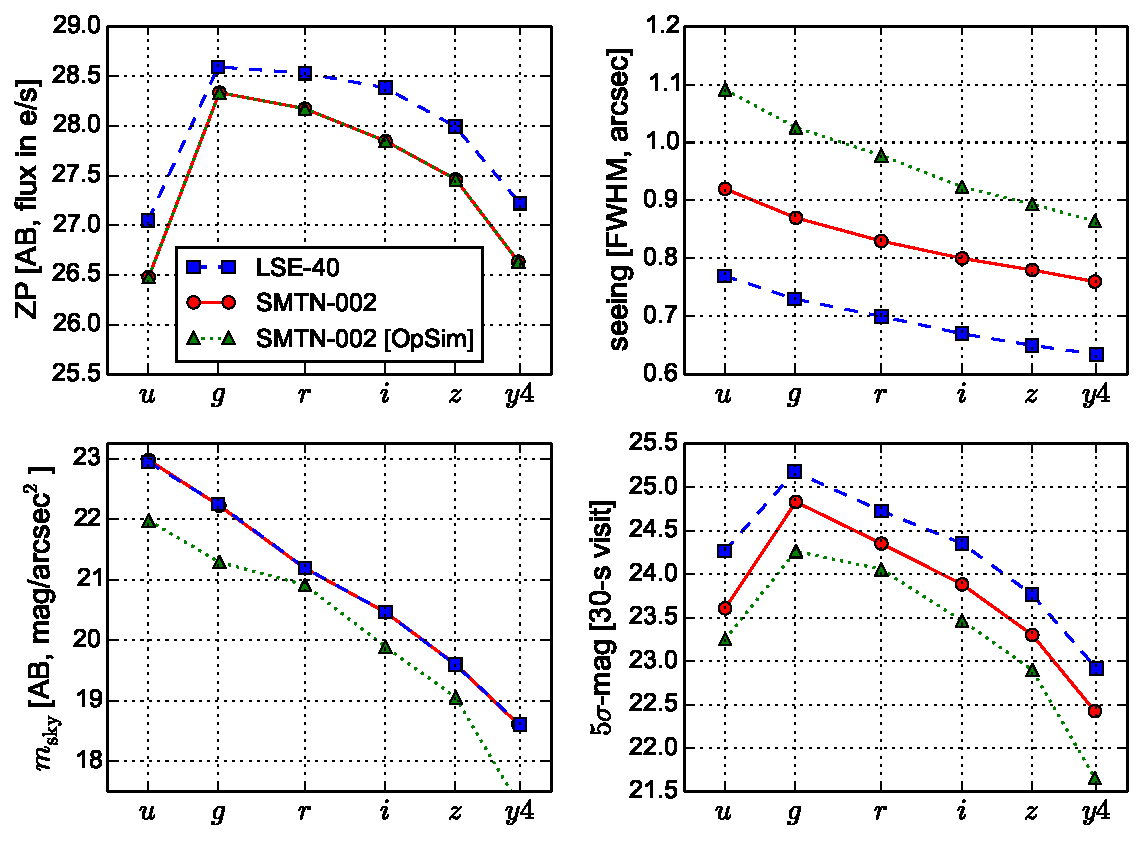
\includegraphics[width=\linewidth]{lsst_model_summary.pdf}
\caption{Zero-points, median seeing, dark sky mags and limiting mags, from (REF REF REF)}
\label{fig:zp}
\end{center}
\end{figure}

\subsection{Simulated SNe}
\label{ssec::snsim}
We use \code{SnSim} to produce the observed SNe Ia and their light curves with the cadence and observing conditions detailed in the previous parts.
Our study is performed for 1 year of wide and 4 years of deep layers.
The repartition in reshift of the simulated SNe Ia is shown in Figure \ref{fig:z_distrib}. We used 4 years of deep and 1 year of wide to get the same number of SNe.
\begin{figure}[ht]
  \centering
  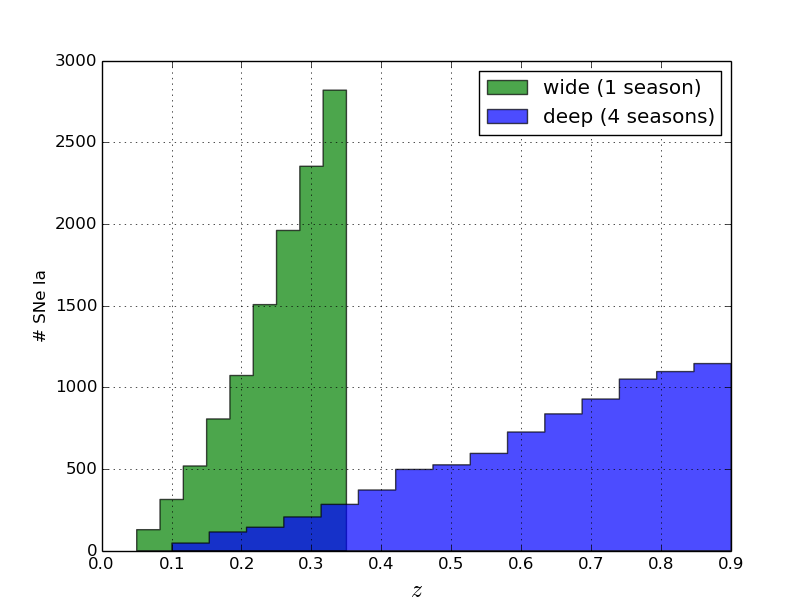
\includegraphics[width=0.7\linewidth]{z_surveys_population.png}
  \caption{Redshift distribution of the SNe Ia simulated with 4 years of deep layer and 1 year of wide for a total of $\approx 20\times10^3$ SNe Ia}
  \label{fig:z_distrib}
\end{figure}
For each type of survey, we show in Figure \ref{fig:lc_examples} that the simulated light curves are well constrained.


Le machin a été produit par SnSim : montrer les jolies LC; très très brève description de SnSim: c'est rapide et c'est chouette \\
Montrer la distribution en redshift des SNe Ia bien mesurées en utilisant les la stratégie d'observation de \ref{subsec::cadence} \\
Plots d'évolution de $\sigma_C$ et $\sigma_{X1}$

\begin{figure*}[t]
\begin{center}
\subfigure[$z = 0.06$]{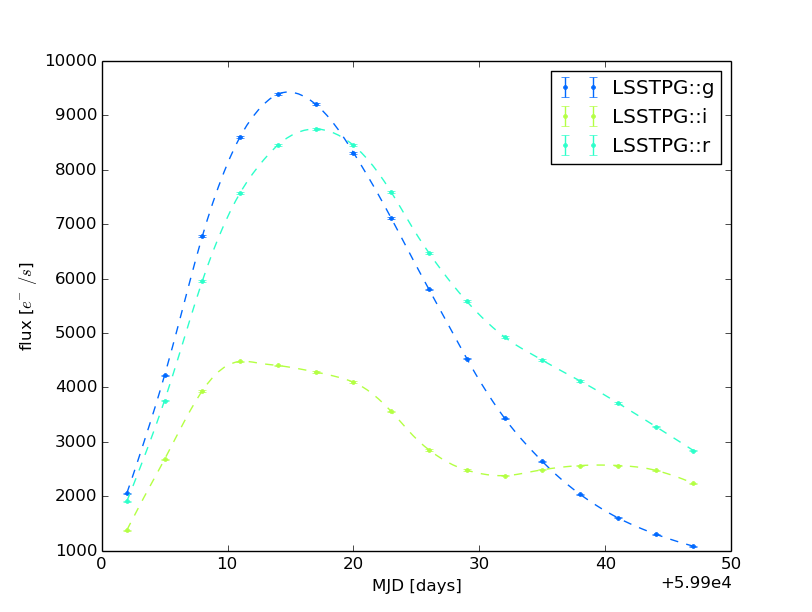
\includegraphics[width=0.48\linewidth]{lc_sn_z006.png}}
\subfigure[$z = 0.87$]{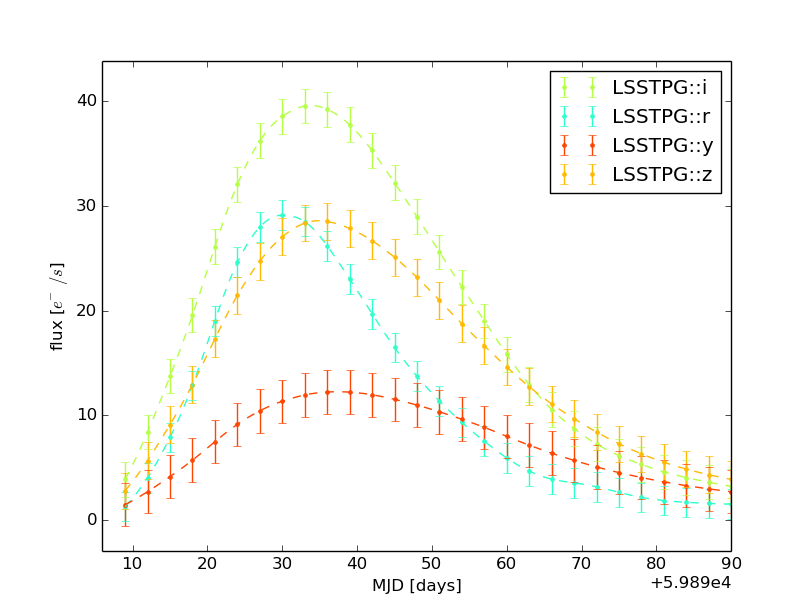
\includegraphics[width=0.48\linewidth]{lc_sn_z087.png}}\\
\caption{caption}
\label{fig:lc_examples}
\end{center}
\end{figure*}

Finally, we show in Figure \ref{fig:sigmas} that in each layer the color $c$, the time of maximum luminosity $t_0$ and the stretch of the simulated SNe Ia are well constrained over their redshift range.

\begin{figure*}[t]
\begin{center}
\subfigure[wide]{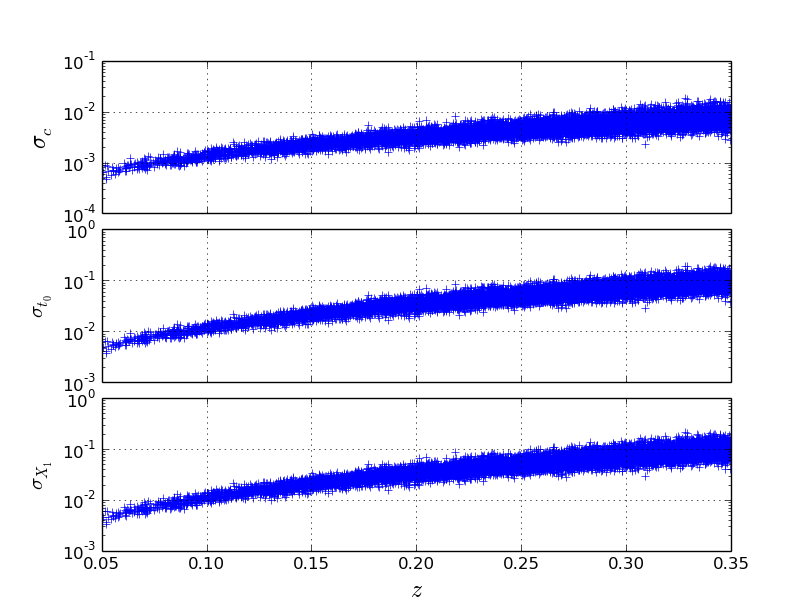
\includegraphics[width=0.48\linewidth]{sigmas_wide.png}}
\subfigure[deep]{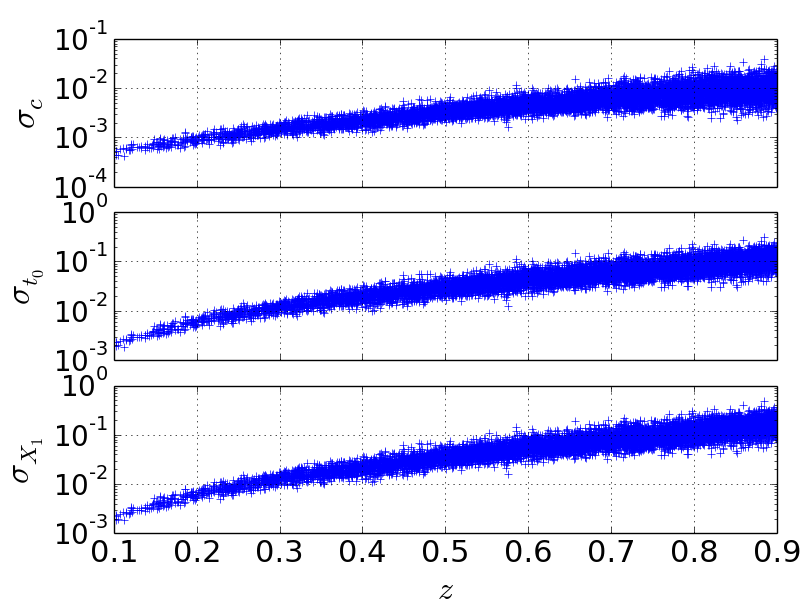
\includegraphics[width=0.48\linewidth]{sigmas_deep.png}}\\
\caption{caption}
\label{fig:sigmas}
\end{center}
\end{figure*}

% ----------------------------------------------------------------------

\section{Analysis Model}
\label{sec::analysis_model}

\subsection{Model details}
\label{subsec::model_details}
In a first time we decide to simplify our model by taking only the flux of our SNe at the day of maximum luminosity in restframe B-band.
To describe simultaneously the flux emitted by all our generated sample of SNe in each band at DayMax we choose to work in astronomer magnitudes for the model to be more linear.
We modelize the observer frame magnitude of the supernova at a redshift $z$ in a band $b$ as follows:
\begin{equation}
\label{eq::raw_model}
 m_b = M_X + 25 + \mu(z, \theta_\text{cosmo}) + 2.5log_{10}(1+z) - 2.5log(\int \lambda S(\lambda) T_b(\lambda) d\lambda) 
\end{equation}
where $M_X$ is the spectrum normalization factor in astronomer logarithm, $\mu(z, \theta_\text{cosmo})$ is its distance modulus related to the luminosity distance $d_L$ as $\mu(z, \theta_\text{cosmo}) = 5log_{10}(d_L)$.
$S(\lambda)$ is the SED of a standard SN Ia that describes its restframe spectrophotometric evolution with wavelength and $T(\lambda)$ is the instrument transmission.
Because of the high statistics brought by the LSST SN survey and its good coverage in a redshift range between $z=0.05$ and $z=0.9$ and to enhance the linearity of our model, we choose to perform a Taylor expansion around the mean position of the passband:

\begin{equation}
\begin{split}
\int \lambda S(\lambda) T_b(\lambda) d\lambda &= \int \lambda \left(S(\bar\lambda)+\frac{\partial S(\bar\lambda)}{\partial \lambda} \times ( \lambda - \bar\lambda ) \right) T_b(\lambda) d\lambda \\
&= S(\bar\lambda) \int \lambda T_b(\lambda) d\lambda + \frac{\partial S(\bar \lambda)}{\partial\lambda} \int \lambda (\lambda - \bar\lambda) T_b(\lambda) d\lambda
\end{split}
\end{equation}

If we choose $\bar \lambda$ to be:

\begin{equation}
  \bar \lambda = \frac{\int \lambda^2 T_b(\lambda) d\lambda}{\int \lambda T_b(\lambda) d\lambda}
\end{equation}

The first order terms are set to zero, so we have:
\begin{equation}
\int \lambda S(\lambda) T_b(\lambda) d\lambda = \int \lambda S(\lambda) T_b(\lambda) d\lambda
\end{equation}

Thus our model in eq \ref{eq::raw_model} becomes:
          
\begin{equation}
  m_b = M_X + 25 + \mu(z, \theta_\text{cosmo}) + 2.5log_{10}(1+z) - 2.5 log_{10} S(\bar \lambda) + \mathcal{Z}_b
\end{equation}

where $\mathcal{Z}_b = -2.5 log \int \lambda T_b(\lambda) d\lambda$ is the band zeropoint.

As we will show later, care must be taken while modelizing the spectrophotometric evolution of the supernovae and its characterization shall remain free to evolve with the input data.
We choose to use a simplified version of the SALT2 model (REF REF REF).
This model incorporates on one side the "astronomers" logarithm of the mean restframe spectrum of a "standard" SN Ia $P(\lambda)$ through a decomposition over a third order B-Spline decomposition and on the other a color law accounting for the color variation of each SN $Q(\lambda)$ that is a polynomial of fourth degree.
Incorporated to the model it gives:

\begin{equation}
m_b = M_X + 25 + \mu(z, \theta_\text{cosmo}) + 2.5log_{10}(1+z) + P(\frac{\bar \lambda}{1+z}) + cQ(\frac{\bar \lambda}{1+z})+ \mathcal{Z}_b
\end{equation}

where the $(1+z)^{-1}$ factors account for the switch to observer frame and $c$ is the color associated to each supernova.


Once the spectrophotometric model has been correctly parametrized, we have to add the standardisation parameters that will ensure the smallest dispersion of our dataset.
Since we do not work in the phase space of the light curves the only standardization parameter we use, still according to the SALT2 model is the brighter-bluer parameter $\beta$.
It incorporates to our model as follows:
\begin{equation}
\label{eq::model}
m_b = M_X + 25 + \mu(z, \theta_\text{cosmo}) + 2.5log_{10}(1+z) + P(\frac{\bar \lambda}{1+z}) + cQ(\frac{\bar \lambda}{1+z}) + \textcolor{red}{c\beta}+ \mathcal{Z}_b
\end{equation}

% ----------------------------------------------------------------------

\subsection{Calibration parameters}
\label{sec::calib_uncertainties}
The core of this work is about how we handle the calibration errors and incorporate them in \ref{eq::model}.
We choose to parametrize them in two different subsets of parameters:
\begin{itemize}
\item $\delta zp$'s, that takes into account the error we make on the normalization of the transmission in each band.
There is one associated to each filter we use.
\item $\delta \lambda$'s, which is the error made in observer frame on the wavelength position of each filter. 
\end{itemize}

Our model then becomes :
\begin{equation}
m_b = M_X + 25 + \mu(z, \theta_\text{cosmo}) + 2.5log_{10}(1+z) + P(\frac{\bar \lambda + \textcolor{red}{\delta\lambda_b}}{1+z}) + cQ(\frac{\bar \lambda + \textcolor{red}{\delta\lambda_b}}{1+z}) + {c\beta} + \mathcal{Z}_b + \textcolor{red}{\delta zp_b}
\end{equation}
These calibration parameters are assiociated to a calibration covariance matrix $C_s$.
In the first order we could consider this matrix as diagonal:
\begin{equation}
C_s = 
\begin{pmatrix}
   \sigma^2_{\delta zp_{g}} & \ & \ & \ & \ & \ \\
   \ & \ddots & \ & \ & \ & \ \\
   \ & \ & \sigma^2_{\delta zp_{y}} & \ & \ & \ \\
   \ & \ & \ & \sigma^2_{\delta\lambda_{g}} & \ & \ \\
   \ & \ & \ & \ & \ddots & \ \\
   \ & \ & \ & \ & \ & \sigma^2_{\delta\lambda_{y}}
\end{pmatrix}
\end{equation}
But it is obvious that non-diagonnal terms should rise depending on the calibration strategy.
The state of the art concerning SNe Ia flux measurements consists in comparing their flux directly with calibrated astrophysical standards.
This way of measuring flux leads to the fact that if we make an error on the wavelength position of the filters, the flux integration of the standard will not be what we should expect and thus leads to an error on the zeropoint of the band.
This phenomenon raise correlation terms between $\delta \lambda$ and $\delta zp$ for a same band.
If we define $\frac{d \delta zp}{d \delta \lambda}$ as the change in zeropoint for $1 \AA$ of filter position error, we obtain it by comparing the integrated flux of a standard (P330E in this case) in a filter and in a shifted filter.

In practice we measure a flux $\phi$ from a object of spectrum $S$ with an instrument of transmission $T$ as:
\begin{equation}
\phi = \int T(\lambda) S(\lambda) \lambda d\lambda + n
\end{equation}
We put the values in Table \ref{tab::calib_derivatives}, then $C_s$ becomes :
\begin{equation}
\label{eq::cov_calib}
C_s = 
\begin{pmatrix}
  \sigma^2_{\delta zp_{g}} + (\sigma_{\delta\lambda_g} \frac{d\delta zp_g}{d\lambda_g})^2 & \ldots & 0 & \frac{d \delta zp_g}{d \delta \lambda_g} \sigma^2_{\delta \lambda_g} & \ldots & 0 \\
   \vdots & \ddots & 0 & \vdots & \ddots & 0 \\
   0 & 0 & \sigma^2_{\delta zp_{y}} + (\sigma_{\delta\lambda_y} \frac{d\delta zp_y}{d\lambda_y})^2 & 0 & 0 & \frac{d \delta zp_y}{d \delta \lambda_y} \sigma^2_{\delta \lambda_y} \\
   \frac{d \delta zp_g}{d \delta \lambda_g} \sigma^2_{\delta \lambda_g} & \ldots & 0 & \sigma^2_{\delta\lambda_{g}} & \ldots & 0 \\
   \vdots & \ddots & 0 & \vdots & \ddots & 0 \\
   0 & 0 & \frac{d \delta zp_y}{d \delta \lambda_y} \sigma^2_{\delta \lambda_y} & 0 & 0 & \sigma^2_{\delta\lambda_{y}}
\end{pmatrix}
\end{equation}

\begin{table*}[t]
\begin{center}
\caption{$\delta zp$'s derivatives with $\delta\lambda$'s computed using P330E spectrum.}
\label{tab::calib_derivatives}
\begin{tabular}{l|ccccc}
\hline
\hline
  & $g$ & $r$ & $i$ & $z$ & $y$ \\
\hline 
  $\frac{d \delta zp}{d \delta \lambda}$ $(mmag/\AA)$& 0.026 & 0.18 & 0.24 & 0.23 & 0.22\\
\hline
\end{tabular}
\end{center}
\end{table*}

% ----------------------------------------------------------------------

\subsection{Model degeneracies}
\label{sec::model_deg}

At this current stage our model have some degeneracies that we must get rid of.
The way to handle this degeneracies is to add priors to our model.
If $J$ is the matrix of the derivatives  of our model with respect to all free parameters (columns) for all light curve amplitudes measured (lines), we can vertically add matrices to $J$ for each prior, corresponding to one or more "additionnal" measurements:
\begin{equation}
J =
\begin{pmatrix}
  J \\
  J_\text{priors}
\end{pmatrix} 
\end{equation}

In parallel, if $C$ is the covariance matrix of our measurements, we add diagonally the covariance matrix of the prior to $C$:
\begin{equation}
C =
\begin{pmatrix}
  C & 0 \\
  0 & C_\text{priors}
\end{pmatrix} 
\end{equation}

In our case we add the following priors:
\begin{itemize}
\item The spectrum normalization, to cut degeneracy with the distance modulus $\mu$ that could increase while $M_X$ decrease.
\item The spectrum color, that is degenerate with the color law ??????????????
\item The fact that the color law is fixed at $\lambda_B$ and $\lambda_V$ respectively mean wavelength of the $B$ and $V$-bands
\item We fix the dispersion of the $M_X$'s at 14\% because otherwise we have degeneracies with the distance moduli.
\item Since we use a $w_0w_a$ cosmology, $\theta_\text{cosmo} = \{ \Omega_m$, $\Omega_k$, $w_0$, $w_a$, $H_0$, $\Omega_bh^2 \}$, we add a Planck prior, extracted from (REF REF REF Planck 2015) results, which brings us the information on $H_0$ and $\Omega_k$ we wouldn't get with the SNe Ia only.
\end{itemize}


% ----------------------------------------------------------------------

\subsection{Error propagation}
\label{sec::linalg}

If we linearize our model $\mathcal{M}$, we have:
\begin{equation}
\mathcal{M} = J \times \vec\theta
\end{equation}
Where $J$ is called the "jacobian" matrix and contains the derivatives of our model with respect to all free parameters (columns) for all light curve amplutude measured (lines) and $\vec\theta$ the vector of all our free parameters.
Lets make review of our free parameters, if $N$ is the number of supernovae measured we have:

\begin{table*}[t]
\begin{center}
\caption{Summary of our model free parameters}
\begin{tabular}{l|ccccccccc}
\hline
\hline
Free parameters & $M_X$ & $\theta_\text{cosmo}$ & $\theta_P$ & $\theta_Q$ & $c$ & $\beta$ & $\mathcal{Z}$ & $\delta zp$ & $\delta \lambda$ \\
\hline
\# parameters & $N$ & 6 & 31 & 5 & $N$ & 1 & 5 & 5 & 5 \\
\hline
\end{tabular}
\end{center}
\end{table*}


We will perform a simultaneous fit of all this parameters, but has we can see there's a lot of them, so to ensure a quicker execution and avoid memory issues we work with sparse matrices.

The fit is performed by minimizing the following $\chi^2$:
\begin{equation}
\chi^2 = \sum_{sb}\frac{[m_{sb} - \mathcal{M}(s, b, \vec\theta)]^2}{\sigma_{sb}}
\end{equation}
The normal equation for this $\chi^2$ is:
\begin{equation}
J^TC^{-1}J = J^TC^{-1}y
\end{equation}
where $C$ is the covariance matrix of the measurements.

Finally we add the calibration covariance matrix $C_s$ (explicited in \ref{sec::calib_uncertainties}) as a prior to our model (as in \ref{sec::model_deg}), since the uncertainties on the $\delta zp$'s and the $\delta \lambda$'s will be evaluated in experiments like StarDICE. For the moment we have to keep in mind that these value are not fixed, and we are going to make this study for several examples of what would be the calibration accuracy for the LSST SN survey.

Since we want to study the performances of the survey, we do not need to perform a fit.
The relevant quantity is the Fisher matrix, that we call $H$
\begin{equation}
H = J^TWJ
\end{equation}
where $W = C^{-1}$.
The inverse of $H$ is the covariance matrix of all the free parameters. It is why we do not have to perform a fit to study the performances of the survey.

% ----------------------------------------------------------------------

\section{Results}
\label{sec::results}
We study the performances through the FoM, we have:
\begin{equation}
FoM = \frac{1}{\sqrt{det(cov(w_0, w_a))}}
\end{equation}
We can then only perform a block inversion of H (se REF REF REF annexe).
We modify the calibration strategy by changing the $\sigma_{\delta \lambda}$'s and the $\sigma_{\delta zp}$'s in $C_s$ (eq \ref{eq::cov_calib}) which is included in $H$ through $W$.
In a first time we vary a same value for all the $\sigma_{\delta zp}$'s while we fix the $\delta \lambda$'s.
We compute the $FoM$ for each common value of the $\sigma_{\delta zp}$'s, we present this result in Figure \ref{fig:fom_zp}.
On this figure we an see that a transition in the level of performances occurs around $\sigma_{\delta zp} = 10^{-3}$.
If we consider that the current uncertainties on the $\delta zp$'s is around $5 \times 10^{-3}$ (JLA), we note that we need improvements to extract the most information from the statistics granted by one year of the survey.

\begin{figure}[ht]
  \centering
  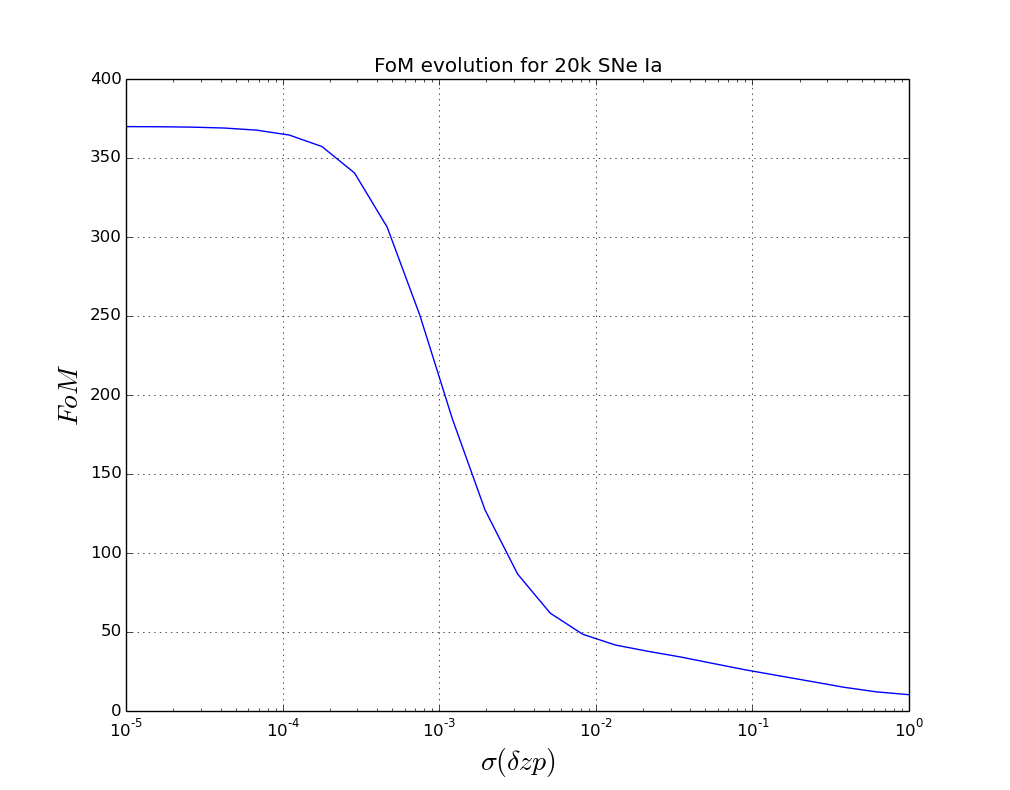
\includegraphics[width=0.7\linewidth]{FoM_20k.png}
  \caption{Evolution of the $FoM$ with the uncertainty on the $\delta zp$'s.}
  \label{fig:fom_zp}
\end{figure}

% ----------------------------------------------------------------------

\section{Discussion}
\label{sec:discussion}
As a parallel work, we wanted to study what would be this results without the training of our spectrophotometric model, that is by not considering $\theta_P$ as free parameters.
The figure \ref{fig:fom_wout_training} shows that, compared to what we obtain with the training, we are making a large overestimation of the performances of the survey, and we would think that the calibration does not need to be that precise. That is why we have to take care with handling the spectrophotometric model.
\begin{figure}[ht]
  \centering
  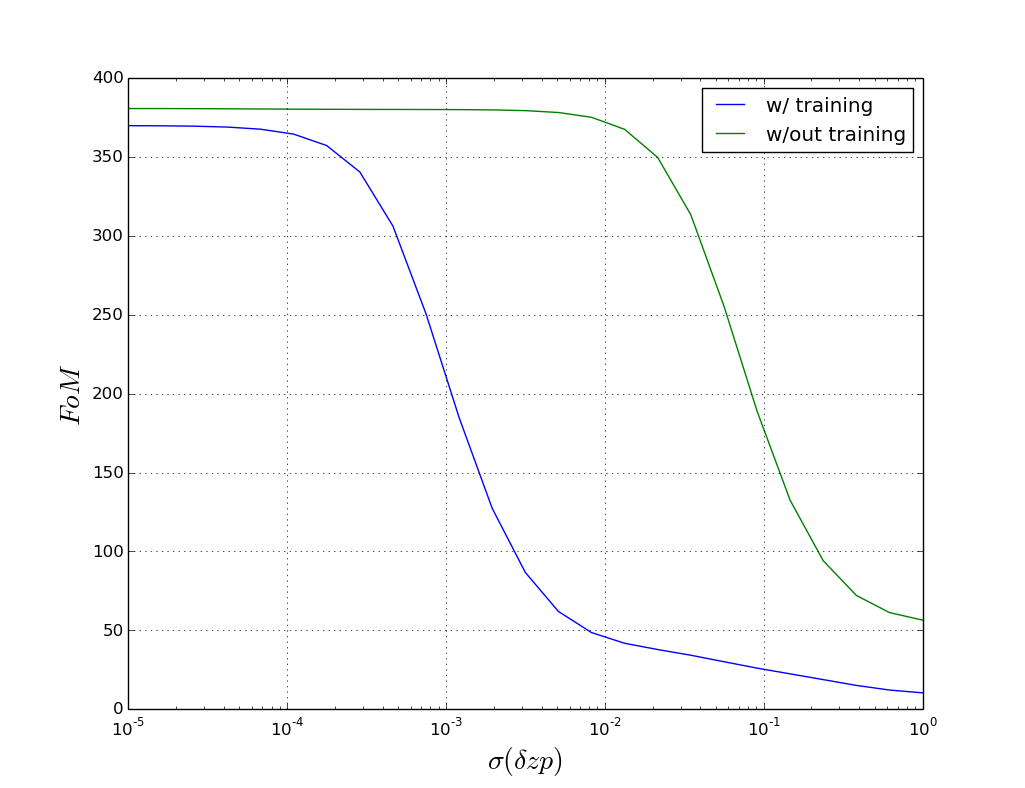
\includegraphics[width=0.7\linewidth]{FoM_20k+training.png}
  \caption{Evolution of the $FoM$ with the uncertainty on the $\delta zp$'s with and without the spectrophotometric model training}
  \label{fig:fom_zp}
\end{figure}


% ----------------------------------------------------------------------

\section{Conclusions}
\label{sec:conclusions}

Here's a summary of what we just reported.

We can draw the following well-organized and neatly-formatted conclusions:
\begin{itemize}
  \item This is important.
  \item We can measure some number with some precision.
  \item This has some implications.
\end{itemize}

Here are some parting thoughts.


% ----------------------------------------------------------------------

\subsection*{Acknowledgments}

Here is where you should add your specific acknowledgments, remembering that some standard thanks will be added via the \code{acknowledgments.tex} and \code{contributions.tex} files.

% 
This is the text imported from \code{acknowledgments.tex}, and will be replaced by some standard LSST DESC boilerplate at some point.
% 


\input{contributions}

%{\it Facilities:} \facility{LSST}

% Include both collaboration papers and external citations:
\bibliography{lsstdesc,main}

\end{document}
% ======================================================================
% 
